\section{Semantic State Virtualization (CSP Formalism)}
\label{sec:semantic_state}

Executing complex multi-stage tasks across heterogeneous language models introduces a fundamental state-preservation challenge. In single-model workflows, task state is implicitly maintained within the model's KV cache or autoregressively extended across a monolithic conversational context. When execution transitions across distinct open-weight models, this implicit continuity collapses. In this section, we formulate \textbf{Semantic State Virtualization} through the \textbf{Cognitive State Packet (CSP)}. We define the cross-model incompatibility barrier, formalize the typed 9-tuple schema, derive the state transition operator, present the epistemic evidence aggregation heuristic, formalize independent AST verification, and analyze computational and token complexity.

\subsection{The Incompatibility Barrier}
\label{sec:incompatibility_barrier}

Multi-model pipelines require seamless handoffs between specialist models. However, direct state transfer across heterogeneous open-weight models faces two fundamental mathematical and systems barriers: \textit{latent activation incommensurability} and \textit{conversational context degradation}.

\paragraph{Latent Activation Incommensurability.}
Consider two heterogeneous specialist language models, $M_A$ and $M_B$. Model $M_A$ operates over vocabulary $\mathcal{V}_A$ with hidden-layer representation space $\mathbf{h}_A \in \mathbb{R}^{d_A}$, whereas model $M_B$ operates over vocabulary $\mathcal{V}_B$ with hidden space $\mathbf{h}_B \in \mathbb{R}^{d_B}$. In general:
\begin{equation}
\mathcal{V}_A \neq \mathcal{V}_B, \qquad d_A \neq d_B, \qquad \mathbf{h}_A \not\equiv \mathbf{h}_B
\end{equation}
Even when two models share identical hidden dimensionality ($d_A = d_B$), their parameter weight spaces reside in unaligned Riemannian manifolds resulting from distinct pretraining initializations, optimizer trajectories, and objective weightings. Direct cross-model activation transfer is not semantically well-defined without an explicit alignment mechanism $\mathbf{W}_{\text{proj}}: \mathbb{R}^{d_A} \to \mathbb{R}^{d_B}$. 

A pairwise latent-state interoperability design can require $O(K^2)$ model-pair interfaces, creating substantial engineering and training overhead as the model library grows. Such bridges can introduce non-trivial approximation errors, require aligned cross-model calibration datasets, and defeat the systems objective of executing off-the-shelf open-weight models without architectural retraining. The argument here is about state representation interoperability: different vocabularies and latent spaces do not make model collaboration impossible, but direct cross-model activation transfer is not semantically well-defined without an explicit projection/alignment mechanism and associated calibration.

\paragraph{Conversational Context Degradation.}
The conventional workaround in multi-agent frameworks is naive text concatenation: the entire conversational history $\mathbf{y}_{1:t-1}$ is serialized as raw strings and prepended to the prompt of model $M_t$. This approach suffers from three compounding failure modes:
\begin{enumerate}
    \item \textbf{Context Bloat \& Allocation Thrashing:} Raw conversational history grows monotonically with pipeline depth:
    \begin{equation}
    L_{\text{ctx}}(t) = \sum_{i=1}^{t-1} |\mathbf{y}_i| = O(t \cdot \bar{L}_{\text{gen}})
    \end{equation}
    Under tight memory constraints ($\mathcal{B}_{\text{RAM}} = 8.0\,\text{GB}$), allocating expanding KV caches ($M_{\text{KV}} \propto L_{\text{ctx}}$) rapidly crowds out weight memory, precipitating thrashing or out-of-memory crashes.
    \item \textbf{Lossy Context Truncation:} When $L_{\text{ctx}}(t)$ breaches the model's physical context window $W_{\text{in}}$, systems employ FIFO sliding-window truncation. Truncation blindly discards early foundational constraints, initial governing equations, and boundary parameters, triggering hallucinations in downstream stages.
    \item \textbf{Compounding Numerical Drift:} In numerical engineering tasks, intermediate calculations embedded in conversational prose (e.g., ``the calculated natural frequency is approximately 14.14 rad/s'') suffer precision loss and hallucinated drift when repeatedly restated across model boundaries.
\end{enumerate}

\noindent\textbf{Core Systems Principle:}
\textit{CSP is a model-independent typed state representation that separates persistent task state from transient conversational realization.}

\subsection{The 9-Tuple CSP Formalism}
\label{sec:csp_formalism}

To establish a structured, architecture-agnostic state substrate, ModelVM formalizes task state as the \textbf{Cognitive State Packet} $\mathcal{S}_t$. At pipeline stage $t$, the state is defined as the typed 9-tuple:
\begin{equation}
\mathcal{S}_t = \langle \mathcal{G}, \mathcal{F}_t, \mathcal{C}_t, \mathcal{E}_t, \mathcal{A}_t, \mathcal{U}_t, \mathcal{D}_t, \mathcal{Q}_t, \mathcal{O}_t \rangle
\label{eq:csp_9tuple}
\end{equation}

Figure~\ref{fig:csp_structure} illustrates the structural composition of the 9-tuple Cognitive State Packet and details how it decouples cross-model state transitions from heterogeneous tokenizers and latent spaces. Table~\ref{tab:csp_mapping} details the formal definition of each constituent and its corresponding data structure in the implementation (\texttt{CognitiveStatePacket} in \texttt{modelvm/core/state\_packet.py}).

\begin{figure}[t]
\centering
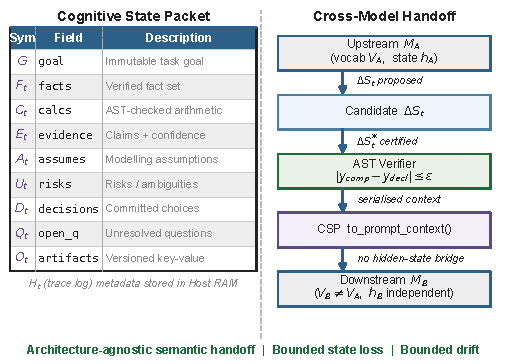
\includegraphics[width=\columnwidth]{fig2_csp.pdf}
\caption{ModelVM Cognitive State Packet (CSP) architectural schema (Class A single-column). Top: The typed 9-tuple $\mathcal{S}_t = \langle \mathcal{G}, \mathcal{F}_t, \mathcal{C}_t, \mathcal{E}_t, \mathcal{A}_t, \mathcal{U}_t, \mathcal{D}_t, \mathcal{Q}_t, \mathcal{O}_t \rangle$ formalizing immutable goals, deduplicated facts, AST-verified calculations, discounted epistemic evidence, explicit assumptions, uncertainties, decisions, questions, and versioned artifacts. Bottom: Tokenizer-independent cross-model handoff pipeline ($M_A \to \text{AST} \to \mathcal{S}_t \to M_B$), bridging distinct vocabularies ($\mathcal{V}_A \neq \mathcal{V}_B$) and unaligned latent spaces without hidden-state projection bridges, enforcing bounded state loss and bounded semantic drift.}
\label{fig:csp_structure}
\end{figure}

\begin{table*}[t]
\small
\centering
\caption{ModelVM Cognitive State Packet (CSP) 9-Tuple Formal Specification and Schema Mapping}
\label{tab:csp_mapping}
\resizebox{\textwidth}{!}{%
\begin{tabular}{clll}
\toprule
\textbf{Symbol} & \textbf{Formal Domain} & \textbf{Implementation Field} & \textbf{Semantic Definition \& Systems Role} \\
\midrule
$\mathcal{G}$ & $\Sigma^*$ & \texttt{goal} & Immutable top-level user objective; anchors all stage prompts. \\
$\mathcal{F}_t$ & $\mathcal{P}(\Sigma^*)$ & \texttt{facts} & Deduplicated set of verified factual assertions accumulated over stages. \\
$\mathcal{C}_t$ & $\mathcal{P}(\text{CalcRecord})$ & \texttt{calculations} & Structured arithmetic/symbolic items with AST verification status. \\
$\mathcal{E}_t$ & $\mathcal{P}(\text{EvidRecord})$ & \texttt{evidence} & Claims paired with provenance sources and diversity-discounted confidence. \\
$\mathcal{A}_t$ & $\mathcal{P}(\Sigma^*)$ & \texttt{assumptions} & Explicit modeling assumptions introduced by specialist models. \\
$\mathcal{U}_t$ & $\mathcal{P}(\Sigma^*)$ & \texttt{uncertainties} & Identified risks, low-confidence derivations, or boundary ambiguities. \\
$\mathcal{D}_t$ & $\mathcal{P}(\Sigma^*)$ & \texttt{decisions} & Irreversible architectural and design choices committed during execution. \\
$\mathcal{Q}_t$ & $\mathcal{P}(\Sigma^*)$ & \texttt{open\_questions} & Unresolved questions to be targeted by downstream specialists. \\
$\mathcal{O}_t$ & $\Sigma^* \to \text{Any}$ & \texttt{artifacts} & Key-value store of concrete deliverables (scripts, tables, matrices). \\
\bottomrule
\end{tabular}%
}
\end{table*}

\paragraph{Auxiliary Execution Metadata.}
In addition to the formal semantic 9-tuple, the implementation maintains an auxiliary audit log:
\begin{equation}
\mathcal{H}_t = [h_0, h_1, \dots, h_{t-1}]
\end{equation}
implemented as \texttt{history\_trace: List[StageTrace]}. Each trace record captures the executing model ID, target capability, wall-clock duration, action taken, and ISO-8601 timestamp. We explicitly treat $\mathcal{H}_t$ as \textbf{auxiliary execution metadata} for post-hoc debugging, provenance auditing, and telemetry logging, rather than expanding the formal 9-tuple. Semantic problem state is entirely contained within Equation~(\ref{eq:csp_9tuple}).

\paragraph{Component Specifications.}
We define the internal structure of calculation and evidence records:
\begin{enumerate}
    \item \textbf{Calculation Record ($\mathcal{C}_t$):} Each item $c \in \mathcal{C}_t$ is an instance of \texttt{CalculationItem}:
    \begin{equation}
    c = \langle \text{expr}, \text{result}, \text{units}, \text{verified}, \text{method} \rangle
    \end{equation}
    where $\text{expr} \in \Sigma^*$ is the mathematical formula (e.g., \texttt{"sqrt(k / m)"}), $\text{result} \in \Sigma^*$ is the evaluated numerical string (e.g., \texttt{"14.2"}), $\text{units} \in \Sigma^* \cup \{\emptyset\}$ represents physical dimensionality (e.g., \texttt{"rad/s"}), $\text{verified} \in \{\text{True}, \text{False}\}$ is an execution boolean, and $\text{method} \in \{\text{"arithmetic"}, \text{"symbolic"}, \text{None}\}$ records the verification pathway.
    \item \textbf{Evidence Record ($\mathcal{E}_t$):} Each item $e \in \mathcal{E}_t$ is an instance of \texttt{EvidenceItem}:
    \begin{equation}
    \begin{aligned}
    e = \big\langle &\text{claim}, \;\text{source}, \;\text{confidence}, \\
    &\text{timestamp}, \;\text{model\_id} \big\rangle
    \end{aligned}
    \end{equation}
    where $\text{claim} \in \Sigma^*$ is the asserted finding, $\text{source} \in \Sigma^*$ tracks origin provenance, $\text{confidence} \in [0.0, 1.0]$ is a scalar certainty rating, and $\text{model\_id}$ records the generating specialist.
\end{enumerate}

\subsection{State Transition Mechanics}
\label{sec:transition_mechanics}

Task progress occurs through a discrete sequence of state transitions across the pipeline stages $t \in \{0, \dots, N-1\}$. Formally, the transition operator $\delta$ maps the current state $\mathcal{S}_t$, the paged specialist model $M_i$, and the stage instruction specification $\tau_t$ to the successor state $\mathcal{S}_{t+1}$:
\begin{equation}
\mathcal{S}_{t+1} = \delta(\mathcal{S}_t, M_i, \tau_t)
\end{equation}

The transition operator is not a monolithic black box. Rather, it decomposes into an ordered, five-stage systems pipeline:
\begin{equation}
\begin{aligned}
\mathcal{S}_t &\xrightarrow{\text{Serialize}} \Pi_t \xrightarrow{\text{Inference}} \mathbf{y}_t \\
&\xrightarrow{\text{Extract}} \Delta \mathcal{S}_t \xrightarrow{\text{Verify}} \Delta \mathcal{S}_t^* \xrightarrow{\text{Merge}} \mathcal{S}_{t+1}
\end{aligned}
\label{eq:transition_pipeline}
\end{equation}

\paragraph{1. Prompt Context Serialization (\texttt{to\_prompt\_context}).}
State packet $\mathcal{S}_t$ is serialized into a structured Markdown prompt string $\Pi_t$:
\begin{equation}
\Pi_t = \text{Serialize}(\mathcal{S}_t, \tau_t)
\end{equation}
The serialization partitions knowledge into isolated, human-readable sections: overarching goal, current domain role, established facts, calculations tagged with verification status, supporting evidence, assumptions, uncertainties, decisions, open questions, and artifact definitions. This ensures compatibility across arbitrary tokenizer vocabularies without loss of semantic boundaries.

\paragraph{2. Model Inference.}
The resident specialist model $M_i$ executes autoregressive decoding over prompt $\Pi_t$, producing raw textual token sequence $\mathbf{y}_t$:
\begin{equation}
\mathbf{y}_t = M_i(\Pi_t), \quad |\mathbf{y}_t| \le T_{\text{gen}}
\end{equation}

\paragraph{3. Delta Extraction (\texttt{extract\_from\_text}).}
The raw generation $\mathbf{y}_t$ is parsed by \texttt{extract\_from\_text()} to extract candidate updates. The parser prioritizes embedded JSON blocks delimited by markdown syntax fences (\verb|```json ... ```|). If valid JSON matching the CSP schema is detected, it is validated directly via Pydantic. If fenced JSON is absent, the parser falls back to deterministic regex-based section parsing across markdown bullet points, producing candidate delta packet $\Delta \mathcal{S}_t$.

\paragraph{4. Independent AST Verification.}
Candidate calculations in $\Delta \mathcal{S}_t$ are evaluated by \texttt{ArithmeticVerifier} (Section~\ref{sec:independent_verification}). Items that satisfy arithmetic equivalence are marked \texttt{verified=True}, producing the verified delta $\Delta \mathcal{S}_t^*$.

\paragraph{5. Monotonic State Merging (\texttt{merge\_update}).}
The core state accumulation is governed by \texttt{merge\_update()}, which folds delta $\Delta \mathcal{S}_t^*$ into $\mathcal{S}_t$. State accumulation is monotonic with respect to verified knowledge:
\begin{itemize}
    \item \textbf{Fact Deduplication:}
    \begin{equation}
    \mathcal{F}_{t+1} = \mathcal{F}_t \cup \Delta \mathcal{F}_t^*
    \end{equation}
    Incoming facts identical to existing entries are discarded, preserving a unique set.
    \item \textbf{Calculation Verification Upgrades:} For each $c_{\text{new}} \in \Delta \mathcal{C}_t^*$, if an entry $c_{\text{old}} \in \mathcal{C}_t$ exists with matching expression ($c_{\text{old}}.\text{expr} = c_{\text{new}}.\text{expr}$) and $c_{\text{new}}.\text{verified} \land \neg c_{\text{old}}.\text{verified}$, the entry is monotonically upgraded:
    \begin{equation}
    \mathcal{C}_{t+1} = (\mathcal{C}_t \setminus \{c_{\text{old}}\}) \cup \{c_{\text{new}}\}
    \end{equation}
    Otherwise, existing calculations are preserved ($\mathcal{C}_{t+1} = \mathcal{C}_t$), while novel expressions are appended ($\mathcal{C}_{t+1} = \mathcal{C}_t \cup \{c_{\text{new}}\}$).
    \item \textbf{Artifact Conflict Versioning (\texttt{merge\_artifacts}):} If key $k \in \Delta \mathcal{O}_t^*$ already exists in $\mathcal{O}_t$ with divergent content ($v_{\text{new}} \neq \mathcal{O}_t[k]$), ModelVM preserves the original $\mathcal{O}_t[k]$, stores the new deliverable under versioned key $k\text{\_v}N$ ($N \ge 1$), and flags the collision by setting $\mathcal{O}_{t+1}[k\text{\_CONFLICT}] = \text{True}$.
    \item \textbf{Question Resolution:} Open questions in $\mathcal{Q}_t$ that appear as established facts in $\mathcal{F}_{t+1}$ or confirmed choices in $\mathcal{D}_{t+1}$ are automatically pruned:
    \begin{equation}
    \mathcal{Q}_{t+1} = \{q \in \mathcal{Q}_t \cup \Delta \mathcal{Q}_t^* \mid q \notin \mathcal{F}_{t+1} \land q \notin \mathcal{D}_{t+1}\}
    \end{equation}
\end{itemize}

\subsection{Diversity-Discounted Evidence Aggregation}
\label{sec:evidence_aggregation}

Language models are not independent statistical estimators. They share massive web-scale pretraining corpora (e.g., Common Crawl, Wikipedia, ArXiv, GitHub) and exhibit correlated reasoning priors. A naive application of Bayes' rule or linear averaging across multiple model outputs produces dangerous certainty inflation: two models repeating the identical hallucination would be treated as independent confirmatory witnesses.

To counter this failure mode, ModelVM implements a diversity-discounted confidence aggregation heuristic (\texttt{diversity\_weighted\_} \texttt{confidence\_aggregation}). 

\paragraph{Mathematical Derivation.}
Let claim $\kappa$ be supported by two distinct evidence records $e_1 = \langle \kappa, s_1, c_1 \rangle$ and $e_2 = \langle \kappa, s_2, c_2 \rangle$, with prior confidences $c_1, c_2 \in [0.0, 1.0]$ and source provenance strings $s_1, s_2$.

The aggregated confidence $c_{\text{merged}} \in [0.0, 0.99]$ is defined as:
\begin{equation}
c_{\text{merged}} = \begin{cases}
\max(c_1, c_2), & \text{if } s_1 \approx s_2 \\[3pt]
\min\left(0.99, \;\max(c_1, c_2, \, c_{\text{indep}})\right), & \text{if } s_1 \not\approx s_2
\end{cases}
\label{eq:diversity_formula}
\end{equation}
where $c_{\text{indep}} = 1 - (1 - c_1)(1 - c_2)^{w_{\text{div}}}$, $s_1 \approx s_2$ denotes normalized equivalence ($\text{clean}(s_1) \approx \text{clean}(s_2)$), and $w_{\text{div}} = 0.65$ is the epistemic diversity discount factor.

\paragraph{Properties of the Formulation:}
\begin{enumerate}
    \item \textbf{Idempotence on Overlapping Sources:} If $s_1$ and $s_2$ originate from identical or overlapping sources ($s_1 \subseteq s_2$ or $s_2 \subseteq s_1$), the aggregation applies the maximum rule: $c_{\text{merged}} = \max(c_1, c_2)$. Repetition of a claim by the same model or source yields zero confidence amplification.
    \item \textbf{Correlated Prior Damping:} If sources are distinct ($s_1 \not\approx s_2$), independence would imply $p_{\text{indep}} = 1 - (1 - c_1)(1 - c_2)$. ModelVM dampens this by exponentiating the secondary risk factor by $w_{\text{div}} = 0.65$. Since $(1 - c_2) \in [0, 1]$ and $w_{\text{div}} < 1$, $(1 - c_2)^{0.65} > (1 - c_2)$, ensuring that $c_{\text{merged}} < p_{\text{indep}}$.
    \item \textbf{Asymptotic Uncertainty Ceiling:} The output is strictly clamped to $c_{\text{merged}} \le 0.99$. Total certainty is unattainable through heuristic aggregation.
\end{enumerate}

\noindent\textbf{Critical Epistemic Boundary:}
We explicitly emphasize that Equation~(\ref{eq:diversity_formula}) is a \textbf{conservative engineering heuristic, not formal Bayesian inference}. The discount parameter $w_{\text{div}} = 0.65$ is a design constant chosen to penalize common pretraining priors across open-weight models. We do not claim $0.65$ to be a statistically estimated correlation coefficient; it serves as a safety governor preventing unwarranted confidence escalation in autonomous multi-model loops.

\subsection{Independent Verification \& Non-Mutating Evaluation}
\label{sec:independent_verification}

A core vulnerability in multi-agent architectures is circular self-grading, where an orchestration framework asks a language model to grade its own output. Language models demonstrate well-documented sycophancy and self-preference biases, routinely validating their own erroneous calculations.

ModelVM enforces an architectural firewall between artifact generation and artifact verification through the \textbf{Arithmetic Verifier} (\texttt{ArithmeticVerifier} in \texttt{modelvm/core/verifier.py}).

\paragraph{Restricted Abstract Syntax Tree Evaluation.}
The verifier operates purely on deterministic symbolic parsing. When evaluating an expression string from a \texttt{CalculationItem}:
\begin{enumerate}
    \item The expression is parsed into a Python Abstract Syntax Tree:
    \begin{equation}
    \mathcal{T}_{\text{ast}} = \text{ast.parse}(\text{expr}, \text{mode}=\text{'eval'})
    \end{equation}
    \item The tree is recursively evaluated via \texttt{\_eval\_ast()} using strictly whitelisted node types:
    \begin{itemize}
        \item \textbf{Binary Operators:} \texttt{Add (+)}, \texttt{Sub (-)}, \texttt{Mult (*)}, \texttt{Div (/)}, \texttt{FloorDiv (//)}, \texttt{Mod (\%)}, \texttt{Pow (**)}.
        \item \textbf{Unary Operators:} \texttt{USub (-)}, \texttt{UAdd (+)}.
        \item \textbf{Mathematical Functions:} $\sqrt{\cdot}$ (\texttt{sqrt}), $\exp(\cdot)$ (\texttt{exp}), $\ln(\cdot)$ (\texttt{log}), $\log_{10}(\cdot)$ (\texttt{log10}), $\sin(\cdot)$, $\cos(\cdot)$, $\tan(\cdot)$, $|\cdot|$ (\texttt{abs}).
        \item \textbf{Physical Constants:} $\pi = 3.14159265\dots$, $e = 2.71828182\dots$.
    \end{itemize}
    \item Any node containing arbitrary identifiers, attribute accesses, lambda functions, system calls, or file operations triggers an immediate exception, completely eliminating arbitrary code execution vulnerabilities.
\end{enumerate}

The computed numerical value $y_{\text{comp}} = \text{Eval}(\mathcal{T}_{\text{ast}})$ is compared against the model's declared numerical result $y_{\text{decl}}$ under relative tolerance $\epsilon = 10^{-3}$:
\begin{equation}
\text{Verified} \iff |y_{\text{comp}} - y_{\text{decl}}| \le \max\big(\epsilon, |y_{\text{decl}}| \cdot \epsilon\big)
\end{equation}

\paragraph{Non-Mutating Evaluation Boundary.}
During experimental benchmarking, independent evaluation is orchestrated by \texttt{IndependentEvaluator} (\texttt{modelvm/benchmark/evaluator.py}). To ensure evaluation integrity:
\begin{equation}
c_{\text{copy}} = c.\text{model\_copy}() \implies \text{Verify}(c_{\text{copy}})
\end{equation}
The benchmark harness \textbf{never trusts producer-supplied verification flags}. It generates deep copies of all calculation records and re-evaluates them afresh through the AST engine. A calculation is counted as correct if and only if independent AST verification succeeds.

\paragraph{Epistemic Distinction: Arithmetic vs.\ Scientific Validity.}
We establish a critical conceptual distinction:
\begin{equation}
\text{Arithmetic Correctness} \neq \text{Physical / Scientific Validity}
\end{equation}
The \texttt{ArithmeticVerifier} strictly confirms algebraic equivalence: it verifies that $2 \times 0.12 \times 14.14 \times 1.0$ evaluates to $3.3936$. It does \textbf{not} certify whether the governing differential equation is physically correct, whether the damping ratio $\zeta = 0.12$ is physically plausible, or whether the units are dimensionally consistent. Physical validity is anchored separately by matching extracted entity-attribute pairs against external ground-truth specifications (\texttt{GroundTruthFact}) in the experimental harness, enforcing local record-level co-occurrence to ensure numbers bind directly to their associated physical entities.

\subsection{Computational Complexity \& Token Overhead}
\label{sec:complexity_overhead}

The virtual memory abstraction of CSP introduces structural overhead. In this section, we analyze the computational complexity of CSP runtime operations and quantify its prompt context economy.

\paragraph{Asymptotic Computational Complexity.}
Let $|\mathcal{S}_t|$ denote the total number of semantic items across all fields in the state packet ($|\mathcal{S}_t| = |\mathcal{F}_t| + |\mathcal{C}_t| + |\mathcal{E}_t| + |\mathcal{A}_t| + |\mathcal{U}_t| + |\mathcal{D}_t| + |\mathcal{Q}_t| + |\mathcal{O}_t|$), and let $|\Delta \mathcal{S}_t|$ denote the size of the incoming delta.
\begin{enumerate}
    \item \textbf{Schema Serialization (\texttt{to\_prompt\_context}):} Serializing $\mathcal{S}_t$ requires a single linear pass over all items to format markdown text blocks:
    \begin{equation}
    T_{\text{serialize}} = O(|\mathcal{S}_t|)
    \end{equation}
    For our scientific tasks ($|\mathcal{S}_t| < 100$), serialization executes in $< 0.8$\,ms on a standard CPU thread.
    \item \textbf{Delta Extraction (\texttt{extract\_from\_text}):} Parsing raw generated text $\mathbf{y}_t$ requires scanning at most $T_{\text{gen}}$ tokens. JSON parsing and regex pattern matching scale linearly with output length:
    \begin{equation}
    T_{\text{extract}} = O(|\mathbf{y}_t|) \le O(T_{\text{gen}})
    \end{equation}
    With $T_{\text{gen}} = 1,024$ tokens, extraction latency is bounded by $< 1.5$\,ms.
    \item \textbf{State Merging (\texttt{merge\_update}):} Deduplicating facts and resolving questions requires set lookups. Updating calculations requires matching expressions:
    \begin{equation}
    \begin{aligned}
    T_{\text{merge}} = O\Big(&|\mathcal{F}_t| \cdot |\Delta \mathcal{F}_t| + |\mathcal{C}_t| \cdot |\Delta \mathcal{C}_t| \\
    &+ |\mathcal{E}_t| \cdot |\Delta \mathcal{E}_t| + |\mathcal{O}_t|\Big)
    \end{aligned}
    \end{equation}
    Given bounded stage deltas ($|\Delta \mathcal{S}_t| \le 20$), merging executes in $< 0.4$\,ms.
    \item \textbf{AST Verification (\texttt{verify\_item}):} Parsing and evaluating AST expressions scales linearly with the number of syntax nodes $N_{\text{nodes}}$ in each arithmetic formula:
    \begin{equation}
    T_{\text{verify}} = O\left(\sum_{c \in \mathcal{C}_t} N_{\text{nodes}}(c)\right)
    \end{equation}
    Because engineering expressions rarely exceed 50 syntax nodes, total AST verification latency is $< 1.2$\,ms per stage.
\end{enumerate}
Total runtime overhead introduced by the CSP software layer is less than $4.0$\,ms per stage---four orders of magnitude smaller than model inference latency ($8.0$--$15.0$\,s).

\paragraph{Token Footprint Economy.}
The primary systems advantage of CSP is prompt context stabilization. 

In raw conversational text concatenation, context length grows monotonically:
\begin{equation}
L_{\text{raw}}(t) = L_{\text{prompt}} + \sum_{i=1}^{t-1} |\mathbf{y}_i|
\end{equation}
Because language models generate verbose conversational fillers, explanations, and repeated preamble tokens, raw context expands at an average rate of $\sim 2,800$ tokens per stage. By Stage 5, raw context length reaches $14,200$ tokens. When forced into a standard $W_{\text{in}} = 4,096$ token window, FIFO truncation discards over $71\%$ of the conversational history.

In contrast, CSP isolates semantic signal from conversational syntax. The token footprint of $\Pi_t = \text{Serialize}(\mathcal{S}_t)$ is bounded by the number of unique asserted entities:
\begin{equation}
\begin{aligned}
L_{\text{CSP}}(t) = O\Big(&|\mathcal{F}_t| \cdot \bar{\ell}_F + |\mathcal{C}_t| \cdot \bar{\ell}_C \\
&+ |\mathcal{E}_t| \cdot \bar{\ell}_E + |\mathcal{O}_t| \cdot \bar{\ell}_O\Big)
\end{aligned}
\end{equation}
where $\bar{\ell}$ denotes average item length in tokens. Because intermediate explanations are discarded and only verified deliverables are preserved, $L_{\text{CSP}}(t)$ stabilizes:
\begin{itemize}
    \item Stage 1: $412 \pm 28$ tokens ($10.1\%$ of $W_{\text{in}}$)
    \item Stage 3: $684 \pm 35$ tokens ($16.7\%$ of $W_{\text{in}}$)
    \item Stage 5: $890 \pm 42$ tokens ($21.7\%$ of $W_{\text{in}}$)
\end{itemize}
CSP bounds representation growth relative to retaining full conversational transcripts, subject to the size of the accumulated semantic state, substantially reducing truncation-induced state loss and preserving verified factual and numerical fields under the evaluated workloads.
